\chapter{Analisi SWOT}
\section{Analisi SWOT di opportunità, minacce, punti di forza e punti di debolezza}

La \textbf{Figura~\ref{fig:swot}} riassume l'analisi SWOT dell'idea progettuale in esame.

\begin{figure}[H]
    \centering
    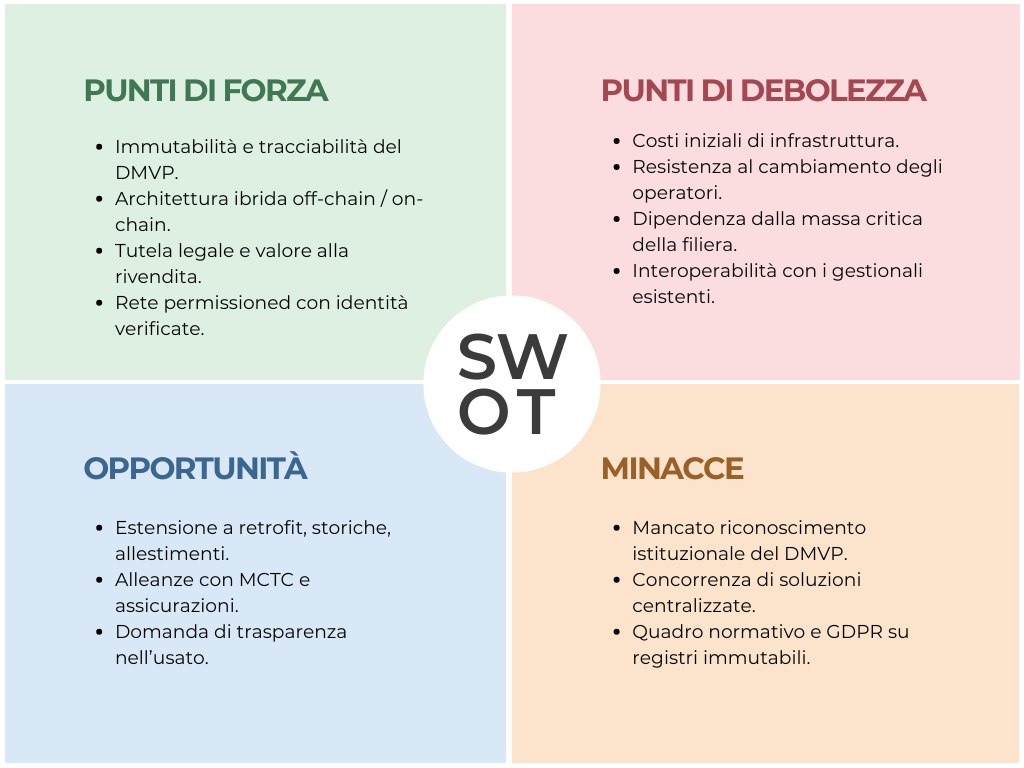
\includegraphics[width=\textwidth]{imgs/swot.png}
    \caption{Analisi SWOT}
    \label{fig:swot}
\end{figure}

L'analisi SWOT mette in luce i punti di forza, le debolezze, le opportunità e le minacce di \textit{Tuning Ledger}, la piattaforma per la gestione del \textit{Digital Modified Vehicle Passport} (DMVP) basata su blockchain permissioned. Di seguito vengono esaminati i principali aspetti che caratterizzano il progetto.

\subsection*{Punti di Forza}
Il sistema offre numerosi vantaggi che ne aumentano il valore e la competitività nel settore dell'automotive tuning. In particolare:

\begin{enumerate}
    \item \textbf{Immutabilità e tracciabilità del passaporto digitale}: grazie all'ancoraggio degli hash sul registro distribuito, ogni fase del ciclo di vita del veicolo modificato -- dalla registrazione del veicolo base alla certificazione delle modifiche -- risulta verificabile e non alterabile. Ciò azzera la possibilità di retrodatare interventi, sostituire documentazione tecnica o dichiarare modifiche mai eseguite.

    \item \textbf{Architettura ibrida off-chain/on-chain}: la separazione tra i dati descrittivi voluminosi (schede tecniche, documentazione fotografica, certificati), conservati nel database off-chain, e le relative impronte crittografiche registrate on-chain consente di coniugare l'integrità garantita dalla blockchain con l'efficienza e la sostenibilità economica dell'archiviazione tradizionale, senza gravare sulle prestazioni della rete.

    \item \textbf{Tutela legale degli attori e valorizzazione del veicolo}: la registrazione immutabile delle lavorazioni costituisce una prova documentale a favore dell'Azienda di Tuning contro contestazioni infondate, riduce il rischio legale della Concessionaria in caso di modifiche non conformi e fornisce al Cliente Privato uno storico certificato che accresce il valore del veicolo al momento della rivendita.

    \item \textbf{Rete permissioned con identità verificate}: l'adozione di una blockchain ad accesso controllato, in cui l'Intermediario verifica preventivamente l'identità di tutti gli attori B2B ammessi, garantisce l'affidabilità della fonte di ogni registrazione e agevola il coinvolgimento di intermediari esperti, capaci di trasferire innovazione digitale verso gli operatori del settore.
\end{enumerate}

\subsection*{Punti di Debolezza}
Nonostante i vantaggi, l'implementazione del sistema presenta alcune criticità che potrebbero limitarne la diffusione e l'adozione da parte degli attori della filiera. In particolare:

\begin{enumerate}
    \item \textbf{Costi di implementazione e infrastruttura}: lo sviluppo della piattaforma, l'esercizio dei nodi della rete permissioned e l'integrazione con i sistemi esistenti richiedono investimenti iniziali elevati, che rappresentano una barriera economica significativa per le officine di tuning di piccole dimensioni e per le realtà artigianali.

    \item \textbf{Resistenza al cambiamento degli operatori}: l'introduzione di procedure digitali strutturate, che impongono la rendicontazione puntuale di ogni lavorazione e componente installato, potrebbe incontrare resistenze da parte di operatori abituati a una gestione informale o cartacea della documentazione tecnica.

    \item \textbf{Dipendenza dalla massa critica della filiera}: il valore della piattaforma cresce con il numero di attori aderenti. Se i Centri di Certificazione o le Concessionarie non partecipassero attivamente, il DMVP resterebbe incompleto e perderebbe la propria funzione di fonte unica e certificata della verità; a ciò si aggiunge una forte dipendenza operativa dall'Intermediario, unico soggetto responsabile della governance della rete.

    \item \textbf{Scalabilità e interoperabilità}: l'integrazione con i sistemi gestionali eterogenei già in uso presso concessionarie, officine ed enti di certificazione, spesso proprietari e non standardizzati, può presentare complessità tecniche in fase di configurazione dei canali di comunicazione.
\end{enumerate}

\subsection*{Opportunità}
L'evoluzione del mercato e l'attenzione crescente verso la trasparenza e la conformità normativa offrono numerose opportunità di crescita e sviluppo per il sistema. In particolare:

\begin{enumerate}
    \item \textbf{Espansione del mercato}: il modello del passaporto digitale può essere esteso oltre il tuning tradizionale verso ambiti affini e in forte crescita, quali il retrofit elettrico, il restauro e la certificazione dei veicoli storici, l'allestimento di veicoli commerciali e la gestione documentale delle flotte aziendali, ampliando in modo significativo il bacino d'utenza.

    \item \textbf{Disponibilità di collaborazioni strategiche}: la possibilità di creare alleanze con la Motorizzazione Civile, con le associazioni di categoria del settore, con le compagnie assicurative e con organizzazioni di promozione della tecnologia DLT aumenta la credibilità del sistema e potrebbe favorirne l'adozione come standard di riferimento per la documentazione delle modifiche.

    \item \textbf{Crescente domanda di trasparenza e conformità}: acquirenti, compagnie assicurative e autorità di controllo richiedono garanzie sempre maggiori sulla storia e sulla regolarità dei veicoli, soprattutto nel mercato dell'usato. Questa tendenza, rafforzata dalla progressiva diffusione dei passaporti digitali di prodotto~\cite{espr}, rappresenta un'opportunità rilevante per il sistema, che risponde in modo nativo a tali requisiti attraverso la certificazione digitale del ciclo di vita del veicolo modificato.
\end{enumerate}

\subsection*{Minacce}
Infine, ci sono alcune minacce esterne che potrebbero ostacolare la diffusione del sistema o limitarne il potenziale complessivo. In particolare:

\begin{enumerate}
    \item \textbf{Mancato riconoscimento istituzionale del DMVP}: in assenza di un valore formale attribuito al passaporto digitale da parte della Motorizzazione Civile e delle compagnie assicurative, il DMVP rischia di configurarsi come un adempimento aggiuntivo rispetto alla documentazione cartacea già obbligatoria, anziché sostitutivo di essa. Ne deriverebbe, per gli operatori della filiera, un costo privo di un ritorno immediato e percepibile, con un conseguente rallentamento dell'adozione volontaria della piattaforma.

    \item \textbf{Concorrenza di soluzioni alternative}: operatori software già consolidati nella gestione delle officine e delle concessionarie potrebbero integrare funzionalità di tracciamento proprietarie e centralizzate, meno costose da adottare; parallelamente, le case automobilistiche potrebbero sviluppare passaporti digitali interni al proprio ecosistema, riducendo temporaneamente il vantaggio competitivo della soluzione decentralizzata.

    \item \textbf{Evoluzione normativa e ostacoli legali}: la disciplina sul valore probatorio delle registrazioni su blockchain è in continua evoluzione a livello nazionale ed europeo, così come i requisiti di omologazione delle modifiche~\cite{cds,dpr495}, che variano tra i diversi ordinamenti. A ciò si aggiunge la tensione tra l'immutabilità del registro e gli obblighi in materia di protezione dei dati personali (in particolare il diritto alla cancellazione previsto dal GDPR), che potrebbe imporre modifiche architetturali complesse e rallentare la diffusione della piattaforma.
\end{enumerate}

\section{Valutazione finale dell'Idea Progettuale}

L'analisi SWOT ha evidenziato numerosi aspetti positivi dell'idea progettuale, supportando la decisione di procedere con lo sviluppo della piattaforma per la gestione del passaporto digitale del veicolo modificato basata su blockchain.

L'immutabilità del DMVP, l'efficienza dell'architettura ibrida off-chain/on-chain e la tutela legale offerta a tutti gli attori coinvolti rappresentano i principali punti di forza del progetto, confermando come esso risponda a una domanda di mercato in crescita e offra valore aggiunto lungo l'intera filiera, con un forte focus sulla conformità normativa e sulla certezza delle informazioni.

Tuttavia, l'analisi delle debolezze e delle minacce ha messo in luce alcuni aspetti critici che dovranno essere superati per garantire il successo della piattaforma. I costi di implementazione iniziali e la resistenza al cambiamento degli operatori, unitamente alla necessità di raggiungere una massa critica di attori aderenti, rappresentano le principali sfide. Per mitigare tali ostacoli sarà necessario incentivare un'adozione progressiva, introducendo interfacce d'uso semplificate e modelli di accesso graduali che permettano una transizione tecnologica sostenibile anche per le realtà di piccole dimensioni.

Inoltre, le opportunità di mercato rappresentano un elemento chiave per il successo del progetto. L'estensione del modello oltre il tuning tradizionale, verso il retrofit elettrico, i veicoli storici e l'allestimento di veicoli commerciali, permetterà di ampliare la base utenti e di aumentare la competitività della piattaforma. Allo stesso modo, collaborazioni strategiche con la Motorizzazione Civile, le associazioni di categoria e le compagnie assicurative potrebbero rafforzare la credibilità del sistema e incentivarne l'adozione su larga scala. Tali collaborazioni costituiscono, in particolare, la principale leva di mitigazione della minaccia relativa al mancato riconoscimento istituzionale del DMVP: solo l'attribuzione di un valore formale al passaporto digitale da parte degli enti competenti e del comparto assicurativo può trasformarlo da adempimento aggiuntivo in strumento sostitutivo della documentazione tradizionale, rendendo il beneficio immediatamente percepibile dagli operatori della filiera.

Infine, un fattore critico da considerare sarà l'evoluzione del quadro normativo relativo all'impiego della blockchain, in particolare per quanto concerne il valore legale delle registrazioni e la conformità al trattamento dei dati personali: questo potrebbe influenzare l'implementazione del sistema in diversi contesti geografici e amministrativi. Per prevenire eventuali ostacoli legali sarà necessario adattarsi dinamicamente ai cambiamenti normativi e garantire la conformità della piattaforma agli standard di tracciabilità e di omologazione vigenti.

La valutazione complessiva del progetto è positiva, nonostante le sfide da affrontare. Le strategie di mitigazione delle debolezze e delle minacce, unite alle opportunità di mercato e ai punti di forza della piattaforma, suggeriscono che lo sviluppo dell'idea progettuale sia vantaggioso.

I prossimi passi dovranno prevedere la realizzazione di un Project Plan dettagliato, con la definizione dell'architettura a componenti e delle fasi di implementazione, e di un Business Plan volto a valutare la sostenibilità economica dell'iniziativa e a massimizzare l'adozione della piattaforma nel settore dell'automotive tuning.